\chapter{Arquitectura y tecnologías}
\label{chapter:arquitectura}

El objetivo de este capítulo es tener una visión global de lo que será nuestro proyecto, antes de entrar en más profundidad en cada una de las partes. El proyecto que presentamos en este documento consta de dos partes bien diferenciadas. Por un lado, una parte que podemos considerar ``de laboratorio'', en la que realizaremos las labores más analíticas sobre los datos disponibles: extracción, procesamiento, estudio y creación de modelos; la cuál presentamos en la sección \ref{section:arq:mod}. Y por otro lado, una parte ``de explotación'', en la que trataremos de poner en valor los resultados de la primera parte en el mundo real y que será tratada en la sección \ref{section:arq:exp}. 


El capítulo se completará con la sección \ref{section:arq:mant}, dedicada al mantenimiento del proyecto una vez llevado a producción y con la sección \ref{section:arqu:tecn}, en la que se describirán a grandes rasgos todas la tecnologías usadas en el proyecto.





\section{Modelado}
\label{section:arq:mod}
La primera parte de nuestro proyecto pretende conseguir el objetivo principal propuesto en  la sección \ref{section:intro:objetivos}, \textbf{clasificar las llamadas}. Para ello tendremos que analizar y entender los datos que poseemos de las transcripciones y posteriormente construir los modelos necesarios (supervisados o no supervisados) que nos permitan clasificar las llamadas.

Para lograr este objetivo necesitaremos disponer de un \textit{datalake} en el que se almacene todo el histórico de transcripciones de las llamadas, ya que para el entrenamiento de muchos modelos será necesario utilizar un amplio histórico para su entrenamiento. Este \textit{datalake} será un sistema de archivos HDFS perteneciente a una plataforma Hadoop Hortonworks. El procedimiento de carga de las transcripciones en HDFS se encuentra ya realizado y queda fuera del alcance del proyecto. Debido a que no tenemos ningún requisito temporal para la ingesta de las transcripciones, este no será un elemento crítico de nuestro proyecto. 

En cuanto a la plataforma que utilizaremos para realizar la analítica, puede ser independiente del entorno de almacenamiento siempre que podamos transferir los datos a la misma. A lo largo del proyecto hemos trabajado con dos entornos diferentes: 

\begin{itemize}
\item Entorno \textbf{Spark}: Ubicado en un clúster Hadoop Hortonworks, nos ha permitido procesar grandes cantidades de datos en un espacio de tiempo muy reducido, gracias a los beneficios de la programación distribuida. Sin embargo, no se trata del entorno ideal para el entrenamiento de modelos, principalmente para modelos  \textit{deep learning}.

\item Entorno \textbf{GPU}s: Una única máquina con diferentes \textit{GPU}s NVIDIA. Este entorno nos ha permitido entrenar los modelos de \textit{deep learning} con una rapidez pasmosa (comparado con los entornos con CPUs). Ha sido la plataforma principal de analítica durante este proyecto, aunque el preprocesado se viera penalizado con respecto al entorno Spark.


\end{itemize}
 

El modelo presentado en nuestra arquitectura es un elemento sometido al cambio y, además de por posibles mejoras en los hiperparámetros o por la tecnología, debe re-entrenarse conforme se vayan recibiendo datos nuevos en el histórico, ya que es lógico pensar que la temática de las consultas variarán a lo largo del tiempo debido por ejemplo al lanzamiento de nuevos productos. 


En los capítulos \ref{chapter:dataset}, \ref{chapter:nosup} y \ref{chapter:super} trataremos en más detalle toda la parte de modelado, desde el análisis de los datos hasta la creación de modelos supervisados y no supervisados.

\section{Explotación}
\label{section:arq:exp}
La segunda parte del proyecto tendrá como meta llevar a producción el resultado de la etapa de modelado. Teniendo en cuenta que uno de nuestros objetivos consiste en clasificar las llamadas en tiempo real,
el primer paso que debemos abordar es seleccionar un modelo de arquitectura de procesamiento en tiempo real de entre las opciones vistas en la sección \ref{section:arte:big:arq}: Lambda y Kappa. Lo que intentamos en este paso, ya que no existe una solución ideal que se adapte a todos los casos de uso, es encontrar la solución que mejor se adapte a nuestro proyecto.


En nuestro caso, disponemos de todas las llamadas en tiempo real, que nos llegarán en forma de eventos. Además cada llamada podrá ser tratada de forma individual y no debemos preocuparnos por eventos que lleguen con retraso. Estos son los motivos principales que nos han llevado a decidirnos por la arquitectura Kappa propuesta por Jey Kreps, debido a la mayor simplicidad tanto a la hora de elaborar la capa de servicio, como a la hora de mantener un único desarrollo \textit{real-time}. 






En la figura \ref{fig:kappa2} podemos ver la arquitectura global de la solución propuesta. Esta arquitectura consta de dos capas principales. Por un lado, una capa de \textit{streaming} o capa rápida donde se realizará todo el procesamiento en \textit{streaming} de las transcripciones de las llamadas conforme vayan llegando. Por otro lado, una capa de servicio que permite a los usuarios explotar la información procesada en la primera capa. 



\begin{figure}[!ht]
	\centering
	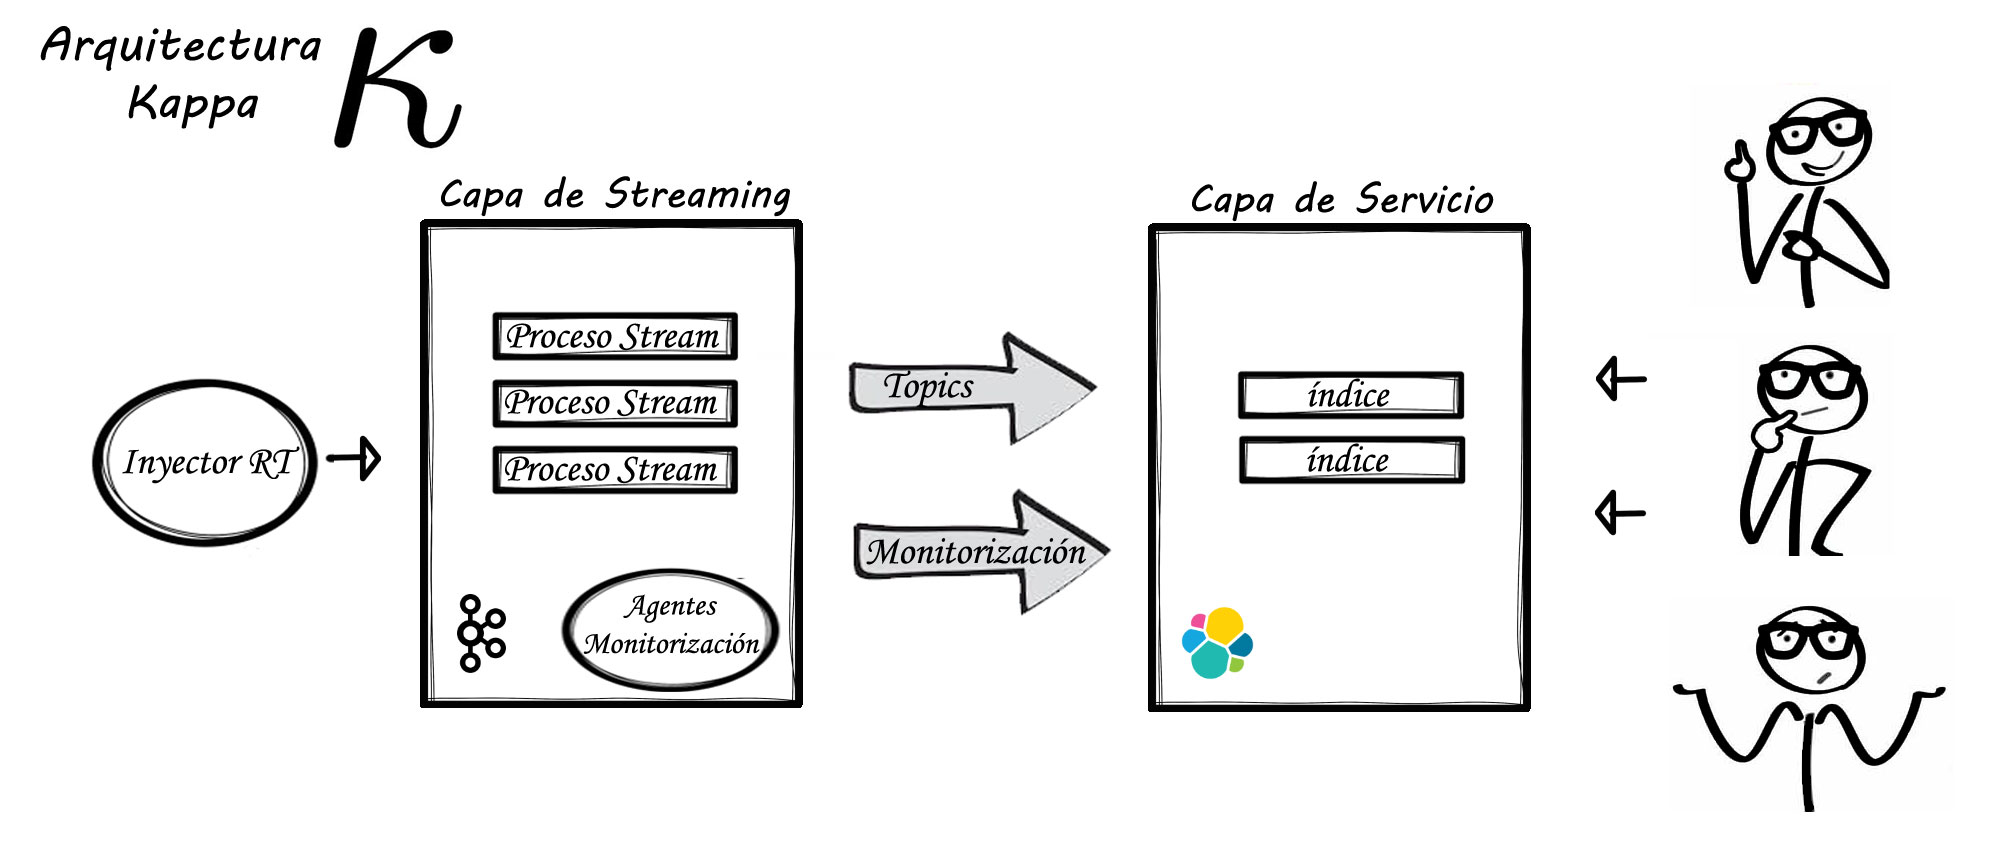
\includegraphics[width=1\textwidth]{images/arqu/kappa_v1}
	\caption{Arquitectura Kappa}
	\label{fig:kappa2}
\end{figure}


El \textit{core} de la primera capa será Apache Kafka, que además nos dará la posibilidad de retener los eventos y poder reprocesarlos en caso de error, siendo una solución ideal para arquitecturas Kappa. De hecho Jey Kreps, quien propuso la arquitectura Kappa es el co-fundador de Confluent, la compañía que se encuentra detrás de Apache Kafka. Los detalles de la capa de \textit{streaming} podemos verlos con más detalle en el capítulo \ref{chapter:prod}.

El núcleo de la capa de servicio será el \textit{stack} de Elastic. Esta solución nos permitirá ingestar los eventos desde la capa rápida en tiempo real y exponerlos a los usuarios. Además usaremos este mismo flujo para todos los eventos de monitorización. El hecho de utilizar el \textit{stack} de Elastic nos dará posibilidad de realizar el alarmado estático y dinámico en esta misma capa.  Los detalles de esta capa se describen en detalle en el capítulo \ref{chapter:servicio}. 




Debido a la situación actual, las llamadas no se ingestan en \textit{real-time} si no que se reciben mediante procesos \textit{batch} cada cierto tiempo. Este escenario cambiará en el futuro por lo que se construirá un elemento de entrada a la capa rápida que actúe como inyector, generando eventos en tiempo real a partir de los datos en \textit{batch}. Esta pieza será suprimida una vez las llamadas sean recibidas en tiempo real. 



\section{Mantenimiento e Integración Continua}
\label{section:arq:mant}

Como ya hemos visto al hablar del entrenamiento del modelo, el desarrollo de este tipo de proyectos no tiene un principio y un final, si no que se trata de un proceso cíclico en el que por necesidades del negocio, por cambio en los datos o por cambio en las tecnologías, será necesario añadir mejoras o modificaciones en nuestro desarrollo. También el despliegue del \textit{software} en producción es un proceso susceptible de futuros cambios.  



Por estos motivos será necesario disponer de algún método para seguir evaluando la calidad del modelo una vez sea llevado a producción,  tener la posibilidad de realizar test A/B en el futuro, y  definir mecanismos que nos permitan, tras cada cambio efectuado, poder realizar las pruebas necesarias y desplegar estos cambios de una manera totalmente automatizada y sin intervención humana.

Para conseguir estos objetivos, con la mayor agilidad posible, será necesario trabajar en un marco de trabajo \textit{DevOps} contando con mecanismos que nos permitan realizar tanto integración, como despliegue continuos.  En el capítulo \ref{chapter:mant} veremos con más detalle como aplicamos esta metodología.





\section{Tecnologías}
\label{section:arqu:tecn}
Al igual que la arquitectura descrita anteriormente era la encargada de responder a las necesidades de negocio, las tecnologías descritas en este apartado nos darán las piezas necesarias para poder construir esa arquitectura y dar respuesta a nuestro caso de uso. 


En el proceso de selección de las tecnologías, no solo se ha tenido en cuenta la idoneidad de las mismas para el caso de uso, si no que se ha valorado también la experiencia en la misma y la disponibilidad dentro del entorno de trabajo. Esto puede provocar que en algunos casos aunque la tecnología se adapte al caso de uso, puedan existir otras soluciones más óptimas cuyo uso era menos viable, dados los plazos de ejecución del proyecto. 

A continuación enumeraremos las tecnologías agrupadas en las diferentes capas que hemos comentado en el apartado de arquitectura, además añadiremos las tecnologías que se usarán para la integración y despliegue continuo. 

\subsection{Modelado}


La parte de modelado la realizaremos trabajando siempre con Python 3.6 y Jupyter, trabajar en un entorno dinámico e interactivo mediante \textit{notebooks} nos dará mucha flexibilidad para poder realizar nuestro análisis.

A continuación vemos las bibliotecas más relevantes que hemos usado, tanto en entorno Spark como en el entorno de GPUs.


\begin{itemize}
	

%	\item \textbf{Spark}: Es un framework de computación en clúster. Este \textit{framework} se encuentra desplegado sobre un clúster Hadoop, específicamente una distribución HortonWorks, y posee librerías específicas para Machine Learning como MLLIB.
%	\item \textbf{Tensorflow} sobre GPUs: Para el entrenamiento de los modelos también disponemos de un cluster con GPUs sobre el que podremos correr código usando la librería de Google Tensorflow para entrenar nuestros modelos.
\item \textbf{Spark SQL y \textit{dataframes}}: Dentro del entorno de Spark, para el procesamiento de los datos trabajaremos con las bibliotecas de Spark SQL y \textit{dataframes}, que nos permitirán de una manera sencilla realizar transformaciones en nuestros datos de forma distribuida.
\item \textbf{MLlib}: También en el entorno de Spark usaremos la biblioteca nativa MLlib, que nos permite crear algoritmos y modelos de \textit{machine learning} sobre un cluster Spark.
\item \textbf{Pandas}: Al igual que en \textit{Spark} utilizamos las bibliotecas de SQL y \textit{dataframes}, Pandas nos permitirá hacer el análisis y manipulación de los datos en cualquier entorno Python.
\item \textbf{ Keras}: Será la biblioteca que usaremos, con  \textbf{Tensorflow} como backend, para crear modelos de \textit{deep learning}.

\item \textbf{Gensim}: Se trata de una biblioteca para el modelado de temas no supervisados y el procesamiento del lenguaje natural.

\item \textbf{NLTK}: Son un conjunto de bibliotecas que nos ayudarán a realizar tareas de procesamiento de lenguaje natural.
\item \textbf{Sklearn}: Se trata de una biblioteca para tareas de \textit{machine learning}, que contiene multitud de funciones que nos ayudarán en nuestro desarrollo.
	
	
\item \textbf{Optuna}:	 Por último, la biblioteca Optuna nos ayudará a optimizar los modelos supervisados que creemos. Hablaremos de ella con más detalle en la sección \ref{section:super:opt}.
	
	
\end{itemize}

\subsection{Explotación}

A continuación veremos las tecnologías y plataformas que harán posible el despliegue de nuestra capa de \textit{streaming}. Estas tecnologías serán vistas con más detalle a lo largo del capítulo \ref{chapter:prod}.

\begin{itemize}
	\item \textbf{Apache Kafka}: Es el \textit{core} de la capa rápida, se trata de un bus de eventos distribuidos, a través del cual se realizará la ingesta o publicación de los eventos (llamadas). Las diferentes capas de procesamiento que requieran estos eventos se suscribirán a este Bus.
	%\item \textbf{Microservicios}: En nuestra capa Real Time construiremos diferentes microservicios en la capa de procesamiento, estos microservicios serán por ejemplo los encargados de devolver los \textit{topics} de cada llamada a partir de una llamada API REST. Estos microservicios correran sobre contenedores en una plataforma Openshift.
	
	
	\item \textbf{Tensorflow Serving}: Servicio para servir modelos de \textit{machine learning} creado dentro del ecosistema Tensorflow.
	\item \textbf{Kafka Stream}: A la hora de procesar la información en eventos ingestada en nuestro Bus Kafka disponemos de Kafka Stream. Una serie de bibliotecas que nos permiten construir aplicaciones y microservicios cuyo origen y destino sean un Bus Kafka. 
	
	\item  \textbf{ Openshift}: Se trata de una plataforma de contenedores de Kubernetes creada por \textit{Red Hat}. Todos los desarrollos de la capa de explotación serán implementados sobre contenedores.

	
\end{itemize}

\subsection{Capa Servicio}

La capa de servicio estará compuesta, como hemos indicado, por el \textit{stack} de Elastic. Este \textit{stack} posee diferentes piezas, cada una de las cuales realiza una función determinada. 

\begin{itemize}

	\item \textbf{Elasticsearch}: Se trata del núcleo del \textit{stack}. Aunque no se trata en el sentido más estricto de una BBDD No-SQL, si no de un motor de búsqueda, Elasticsearch nos permite almacenar la información en forma de documentos json en tiempo real y realizar consultas y agregaciones sobre cualquier campo. Entre las características que podemos aprovechar de Elasticsearch para nuestro objetivo están: 
		\begin{itemize}
			\item Ingesta en tiempo real.
			\item Consulta en tiempo real. 
			\item Disponibilidad de mecanismos de ingesta (Logstash) y consulta (Kibana).
			\item Posibilidad de crear alarmas en base a consultas. 
			\item Posibilidad de crear \textit{jobs} de \textit{machine learning} que detecten anomalías en series temporales. 
			\item API REST: Posibilidad de realizar cualquier operación o consulta mediante API REST.
		\end{itemize}



	\item \textbf{Logstash}: Será la pieza que nos permitirá transportar la información desde la capa de \textit{streaming} a la capa de servicio. Logstash nos permitirá leer de Apache Kafka, realizar las transformaciones necesarias y volcar la información resultante en Elasticsearch. Además de los datos propios de la clasificación, Logtsash nos ayudará a extraer también los datos de monitorización de la capa de Streaming.
	
	\item \textbf{Kibana}: Será el frontal donde los usuarios podrán consultar sus diferentes cuadros de mando y construir nuevos de acuerdo a sus necesidades. También, gracias al módulo de \textit{machine learning} de Elasticsearch, los usuarios podrán crear \textit{jobs} de \textit{machine learning} para detectar anomalías en los temas tratados y generar las alertas necesarias.
	
	
	\item \textbf{Beats}: Se trata de agentes ligeros que nos permitirán extraer información variada de distintas fuentes. En nuestro caso usaremos \textit{Metricbeat} para extraer datos de monitorización de la capa de \textit{streaming}. 
	
	
	
		
	
		
\end{itemize}





\subsection{Integración y Despliegue Continuo}

Por último, para conseguir los objetivos de integración y despliegue continuos utilizaremos diversas  tecnologías. Estas tecnologías, y la interacción entre ellas se verán con más detalle en el capítulo \ref{chapter:mant}.

\begin{itemize}
	\item \textbf{BitBucket}: Será el repositorio usado para almacenar las nuevas versiones de nuestro \textit{software} de manera que podamos tener un control de versiones. Almacenará tanto el código de nuestra capa de \textit{streaming}, como de los modelos que necesitemos poner en producción. 
	\item \textbf{Jenkins}: Es un servidor de integración continua \textit{open source}  que, mediante la creación de tareas, nos ayudará a realizar el \textit{build} de nuestro software realizando de manera automática las pruebas necesarias.
	\item \textbf{Nexus}: Se trata de un gestor de repositorios, en nuestro caso utilizaremos repositorios de Maven. Es usual usar este tipo de gestores de repositorios en las empresas para disponer de bibliotecas propias (y no públicas) y para no tener una dependencia con ningún agente externo.
	\item \textbf{S2I}: Se trata de una funcionalidad de Openshift que será vital para el desarrollo del despliegue continuo. Esta funcionalidad nos permitirá crear nuevas imágenes de contenedores a partir de código o binarios propios.
\end{itemize}










